\documentclass{article}

% if you need to pass options to natbib, use, e.g.:
%     \PassOptionsToPackage{numbers, compress}{natbib}
% before loading neurips_2018

% ready for submission
% \usepackage{neurips_2018}

% to compile a preprint version, e.g., for submission to arXiv, add add the
% [preprint] option:
%     \usepackage[preprint]{neurips_2018}

% to compile a camera-ready version, add the [final] option, e.g.:
     \usepackage[final]{neurips_2018}

% to avoid loading the natbib package, add option nonatbib:
%     \usepackage[nonatbib]{neurips_2018}

\usepackage[utf8]{inputenc} % allow utf-8 input
\usepackage[T1]{fontenc}    % use 8-bit T1 fonts
\usepackage{hyperref}       % hyperlinks
\usepackage{url}            % simple URL typesetting
\usepackage{booktabs}       % professional-quality tables
\usepackage{amsfonts}       % blackboard math symbols
\usepackage{nicefrac}       % compact symbols for 1/2, etc.
\usepackage{microtype}      % microtypography
\usepackage{amsmath}
\usepackage{amssymb}
\usepackage{graphicx}
\usepackage{makecell}
\usepackage{subcaption}
\usepackage{booktabs}

\newcommand{\pd}[2]{\frac{\partial #1}{\partial #2}}
\newcommand{\nl}{\newline}

\title{Deep Learning\\Assignment 3: Deep Generative Models}

% The \author macro works with any number of authors. There are two commands
% used to separate the names and addresses of multiple authors: \And and \AND.
%
% Using \And between authors leaves it to LaTeX to determine where to break the
% lines. Using \AND forces a line break at that point. So, if LaTeX puts 3 of 4
% authors names on the first line, and the last on the second line, try using
% \AND instead of \And before the third author name.

\author{%
  Daniel Daza\\
  University of Amsterdam\\
  \texttt{daniel.dazacruz@student.uva.nl} \\
}

\begin{document}
% \nipsfinalcopy is no longer used

\maketitle

\begin{abstract}
-
\end{abstract}


\section{Variational Autoencoders}

\subsection*{Question 1.1}

\begin{enumerate}
\item Both the AE and VAE can be used to find a code underlying an observation. Ideally, this code should serve as a compressed representation of the input that contains the right amount of information about it, finding a balance that ignores irrelevant details, and keeps meaningful features. In this sense, the models are not different. However, the VAE is a generative model that solves a problem of statistical inference, and it enables the code to have a probabilistic interpretation. For some applications, this can be part of the main function, making it different from the AE. An example of this use is the Bayesian Skipgram \cite{bravzinskas2017embedding}, where words are embedded as probability distributions that capture uncertainty in the representation. This allows to represent ambiguous words with distributions of high variance, and viceversa; and to compute similarities between words via the KL divergence. This would not be possible with the AE, where the code is deterministic and does not have the ability to represent uncertainty.

\item The AE is not generative, because it does not model the data-generating distribution, either explicitly or implicitly. Instead, it finds a deterministic map $\mathbf{z} = f(\mathbf{x})$ for the encoder, and $\mathbf{x} = g(\mathbf{z})$ for the decoder. These functions do not have a probabilistic interpretation, therefore they do not allow for the calculation of likelihoods or expectations.

\item Both the AE and the VAE are trained in an unsupervised way, and the training procedure is based on the reconstruction of the inputs. For this reason, a VAE can be used in place of a standard AE, provided that the additional term for the KL divergence between the approximate posterior and the prior is added to the loss function. For downstream tasks, such as classification, the mean parameterized by the encoder of the VAE can be used in place of the deterministic code provided by the AE.

\item The aspect that enables the VAE to be generative is the ability to define the probability distribution of the latent variable $p(\mathbf{z})$, and the distribution $p(\mathbf{x}\vert\mathbf{z})$ of the observation conditioned on the latent variable. With these components, the VAE learns the joint distribution $p(\mathbf{x},\mathbf{z})$, making it a generative model. A standard AE is only concerned with finding a map to copy the input to the output, and in general it does not have any incentive to find a code that generalizes to unseen observations.
\end{enumerate}

\subsection*{Question 1.2}

According to the graphical model described by the VAE, to obtain a sample of $\mathbf{x}$ we can use ancestral sampling, that is, first we sample the root of the directed graphical model, which in this case corresponds to the latent variable $\mathbf{z}$, and then we use this sample to obtain a sample of its children, corresponding to $\mathbf{x}$. Since we are assuming the pixels to be independent conditioned on $\mathbf{z}$, we only need $\mathbf{z}^{(m)}$ (the $m$-th element of $\mathbf{z}$) to sample $\mathbf{x}^{(m)}$. The sample procedure is then the following:

\begin{align*}
\mathbf{z} &\sim \mathcal{N}(0, \mathbf{I}_D)\\
\mathbf{x}^{(m)} &\sim \text{Bern}(f_\theta(\mathbf{z})^{(m)})\ \forall n = 1, \dots, M
\end{align*}

\subsection*{Question 1.3}

The standard normal prior of the VAE is not a restrictive assumption because samples from it are transformed by the decoding network, $f_\theta(\cdot)$, which can be given arbitrary capacity. We can specify a decoder with a large number of parameters and multiple layers so that it represents a nonlinear transformation representing a map from the simple standard prior, to a sufficiently complicated distribution.

\subsection*{Question 1.4}

\begin{description}
\item[(a)] We can approximate the expectation with a Monte Carlo estimate:
\begin{align*}
\log\int p(\mathbf{x}_n\vert\mathbf{z}_n)p(\mathbf{z}_n)d\mathbf{z}_n &= \log\mathbb{E}_{p(\mathbf{z}_n)}[p(\mathbf{x}_n\vert\mathbf{z}_n)] \\
&\approx \frac{1}{L}\sum_{i=1}^{L} p(\mathbf{x}_n\vert\mathbf{z}_i)
\end{align*}
with $\mathbf{z}_i\sim\mathcal{N}(0, \mathbf{I}_D)$.

\item[(b)] Intuitively, the previous procedure estimates $\log p(\mathbf{x}_n)$ by obtaining a sample of $\mathbf{z}_n$ from the prior, and using it to calculate the probability that the model assigns to $\mathbf{x}_n$. We expect to obtain a good estimate by averaging this probability over multiple sampling steps. The problem with this approach is that values of $\mathbf{z}_n$ where $p(\mathbf{x}_n\vert\mathbf{z}_n)$ assigns a high probability to an observation can lie in a region much smaller than the broad regions that the prior covers. This means that most of the time we will be obtaining samples of $\mathbf{z}_n$ that assign low probability to $\mathbf{x}_n$. Hence, to obtain a good estimate, we will need many samples. This effects worsens as the dimension of $\mathbf{z}$ increases, making the approach very inefficient.
\end{description}

\subsection*{Question 1.5}

\begin{description}
\item[(a)] The smallest KL divergence is obtained when the two distributions are the same. Therefore, if $\mu_q = 0$ and $\sigma_q=1$, $D_{\text{KL}}(q\Vert p) = 0$.
From the definition of the KL divergence, we can see that if for some $x$, $p(x)\rightarrow 0$ and $q(x)>>0$, then $q(x)/p(x)\rightarrow\infty$. We can then make $D_{\text{KL}}(q\Vert p)$ large by letting $\mu\rightarrow\infty$ and $\sigma_q = \mu_q$, so that $q(x)$ assigns high probability to regions where $p(x)$ assigns low probability.

\item[(b)] The KL divergence between a standard prior and a multivariate Gaussian can be found in the original publication \cite{kingma2014vae}. In the univariate case we obtain:
\begin{equation*}
D_{\text{KL}}(q\Vert p) = \frac{1}{2}(\sigma_q^2 + \mu_q^2 - \log(\sigma_q^2) - 1)
\end{equation*}
\end{description}

\subsection*{Question 1.6}

Since the KL divergence is nonnegative, we can write

\begin{align*}
\log p(\mathbf{x}_n) &= \mathbb{E}[\log p(\mathbf{x}_n\vert Z)] - D_{\text{KL}}(q(Z\vert\mathbf{x}_n)\Vert p(Z)) + D_{\text{KL}}(q(Z\vert\mathbf{x}_n)\Vert p(Z\vert\mathbf{x}_n)) \\
&\geq \mathbb{E}[\log p(\mathbf{x}_n\vert Z)] - D_{\text{KL}}(q(Z\vert\mathbf{x}_n)\Vert p(Z))
\end{align*}

Therefore this last expression is a lower bound for the log-probability.

\subsection*{Question 1.7}

If we wanted to optimize the log-probability, we would need to calculate the true posterior distribution $p(\mathbf{z}\vert\mathbf{x})$:
\begin{align*}
p(\mathbf{z}\vert\mathbf{x}) &= \frac{p(\mathbf{z})p(\mathbf{x}\vert\mathbf{z})}{p(\mathbf{x})} \\
&= \frac{p(\mathbf{z})p(\mathbf{x}\vert\mathbf{z})}{\int p(\mathbf{z})p(\mathbf{x}\vert\mathbf{z})d\mathbf{z}}
\end{align*}

The integral in the denominator is not tractable, so we don't have direct access to the posterior.

\subsection*{Question 1.8}
When the lower bound is maximized, this causes the log-probability to increase, and the KL divergence between the approximate and true posteriors to decrease. This means that the model assigns higher probability to the observations, while improving the approximation $q(\mathbf{z}\vert\mathbf{x})$ to be closer to the true posterior $p(\mathbf{z}\vert\mathbf{x})$. This circumvents the problem of an intractable posterior because if the approximate and true posteriors match, maximizing the lower bound will directly maximize the log-probability.

\subsection*{Question 1.9}

If we only use one sample of $\mathbf{z}$, then we have the following loss for a data point: 
\begin{equation*}
-\log p_\theta(\mathbf{x}\vert Z) + D_{\text{KL}}(q_\phi(Z\vert\mathbf{x})\Vert p(Z))
\end{equation*}

To minimize the first term, the model must assign a high probability to the observation $\mathbf{z}$ given the latent variable. If the decoder can use a sample of the latent variable and produce a reconstruction close to the observation, this will mean that the observation is likely under the model. For this reason this loss is also known as the reconstruction loss.

To minimize the second term, the KL divergence between the prior and the approximate posterior must be low. This enforces a constraint in the parameters of the encoder, such that they are free to change in order to create a useful mapping from the observation to the latent variable, but not so much as to deviate from a predefined structure determined by the prior distribution. This term thus acts as a regularizer of the parameters of the model.

\subsection*{Question 1.10}

In the following we will omit the subscript in $\mathbf{x}_n$ as, we will specify the loss for a single sample.

The first step to calculate the loss is to obtain samples of the latent variable from the encoder, to estimate the reconstruction loss. This step comprises a forward pass through the decoder with the observation $\mathbf{x}$ as an input, and a step where $L$ samples of $\mathbf{z}$ are drawn:
\begin{align*}
\boldsymbol{\mu}_e &= \mu_\phi(\mathbf{x}) \\
\boldsymbol{\sigma}_e &= \Sigma_\phi(\mathbf{x}) \\
\mathbf{z}_i &\sim \mathcal{N}(\mathbf{z} \vert \boldsymbol{\mu}_e, \text{diag}(\boldsymbol{\sigma}_e)),\ i = 1, \dots, L
\end{align*}

The samples are then passed through the decoder to obtain the parameters of the Bernoulli distribution:
\begin{equation*}
\boldsymbol{\mu}_{di} = f_\theta(\mathbf{z}_i),\ i = 1, \dots, L
\end{equation*}

We can now estimate the reconstruction loss as follows:
\begin{align*}
\mathcal{L}_n^{\text{recon}} &= -\mathbb{E}_{q_\phi(Z\vert\mathbf{x})}[\log p_\theta(\mathbf{x}\vert Z)] \\
&\approx -\frac{1}{L}\sum_{i=1}^L \log p_\theta(\mathbf{x}\vert \mathbf{z}_i) \\
&=
-\frac{1}{L}\sum_{i=1}^L\log \prod_{m=1}^M \text{Bern}(\mathbf{x}^{(m)}\vert \boldsymbol{\mu}_{di}^{(m)}) \\
&=
-\frac{1}{L}\sum_{i=1}^L\sum_{m=1}^M \mathbf{x}^{(m)}\log\boldsymbol{\mu}_{di}^{(m)} + (1-\mathbf{x}^{(m)})\log(1 -\boldsymbol{\mu}_{di}^{(m)})
\end{align*}

To calculate the regularization term, we can make use of the closed form expression of the KL divergence. Previously we specified it assuming univariate Gaussians, and in the multivariate case we obtain:

\begin{align*}
\mathcal{L}^{\text{reg}} &= \mathcal{} D_\text{KL}(q_\phi(Z\vert\mathbf{x})\Vert p(Z)) \\
&=
\frac{1}{2}\sum_{i=1}^D ((\boldsymbol{\sigma}_e^2)^{(i)} + (\boldsymbol{\mu}_e^2)^{(i)} - \log(\boldsymbol{\sigma}_e^2)^{(i)} - 1)
\end{align*}

\subsection*{Question 1.11}

The gradient of the loss with respect to the variational parameters $\phi$ is required because it contains the information required to update the parameters of the encoder. The encoder influences the loss through the reconstruction, as samples from the approximate posterior are required to obtain the reconstructions. It also affects the loss through the regularization term. Therefore, if we want to optimize the VAE objective, we need to compute $\nabla\mathcal{L}_\phi$.

The problem with obtaining this gradient is that the steps to calculate the loss involve sampling from a probability distribution parameterized by the encoder, which is an operation that is not differentiable with respect to the parameters of the encoder. This can be solved with the reparameterization trick, which consists of obtaining a sample from a distribution that is not parameterized by the encoder, and passing it through a deterministic function such that the result is equivalent to sampling from the approximate posterior. This function is chosen so that it is differentiable with respect to $\phi$, so we can calculate the required gradients.

\subsection*{Question 1.12}

We implemented a VAE following the details outlined in the previous sections. We run experiments on a binary version of the MNIST dataset \cite{lecun1998gradient}, containing black and white images of size 28$\times$28. We use 50,000 images for training and 10,000 for validation.

The encoder of the VAE is a two layer multilayer perceptron (MLP) with 500 units in the first layer. The second layer produces two separate outputs, corresponding to the mean $\boldsymbol{\mu}_e$ and logarithm of the variance $\log\boldsymbol{\sigma}_e^2$ of the approximate posterior. We choose to calculate $\log\boldsymbol{\sigma}_e^2$ instead of $\boldsymbol{\sigma}_e$ to improve numerical stability.

We use 1 sample of the latent variable. For the decoder we use an MLP with two layers, with 500 units in the hidden layer and 28$\times$28 $=$ 784 units in the output layer.

We train the model using the Adam optimizer \cite{kingma2014adam} with a learning rate of 0.001, and a batch size of 128.

\subsection*{Question 1.13}

The mean of the training data with binary images is 0.1306. If for a moment we disregard the effect of the KL divergence, we can estimate the reconstruction loss for a randomly initialized model as follows:

\begin{align*}
\sum_{m=1}^{784} \mathbf{x}^{(m)}\log\boldsymbol{\mu}_d^{(m)} + (1-\mathbf{x}^{(m)})\log(1 -\boldsymbol{\mu}_d^{(m)})
&\approx
\sum_{m=1}^{784} 0.1306\log 0.5 + (1-0.1306)\log 0.5 \\
&\approx 543
\end{align*}

Therefore, the values of the evidence lower bound (ELBO) during training should be below this value.

We show the ELBO for the training and validation set in Figure \ref{fig:vae_curves_a}. As expected, the values are smaller than those of a randomly initialized model. The curves of the ELBO show that the training procedure effectively minimizes the loss in the training and validation sets, indicating that the likelihood of the data has increased under the generative model.

Previous works have observed that in a failure mode of VAEs, the decoder can learn to ignore the latent variable, especially in cases where a flexible decoder can exploit dependencies in the output \cite{bowman2016gensentcontinuous}, such that the KL divergence term of the loss reduces to 0. However, since in our case we are using a model where pixels are independent of each other, this should not be a problem. To verify this, we also show in Figure \ref{fig:vae_curves_b} separately the reconstruction loss and the KL divergence. We observe that at the beginning of training the KL divergence starts at a low value and then increases, showing that the model is driving the approximate posterior away from the prior, which helps to encode meaningful information in the latent variable that the decoder uses to reduce the reconstruction loss.

\begin{figure}[t]
\begin{subfigure}{0.49\textwidth}
\centering
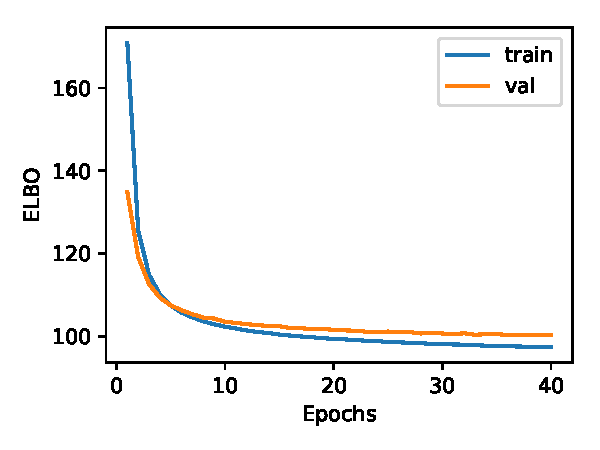
\includegraphics[scale=0.7]{img/elbo.pdf}
\caption{}
\label{fig:vae_curves_a}
\end{subfigure}
\begin{subfigure}{0.49\textwidth}
\centering
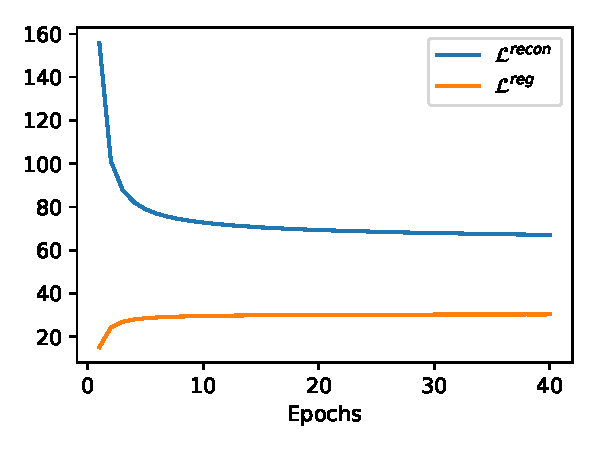
\includegraphics[scale=0.7]{img/recon_reg_losses.pdf}
\caption{}
\label{fig:vae_curves_b}
\end{subfigure}
 \caption{Training curves for the VAE. (a) ELBO for the training and validation sets. (b) Reconstruction loss $\mathcal{L}^{\text{recon}}$ and KL divergence $\mathcal{L}^{\text{reg}}$ on the training set.}
\label{fig:vae_curves}
\end{figure}

\subsection*{Question 1.14}

We take samples from the model before training, halfway through and after training. We obtain these by following the generative procedure, that is, first we sample from the prior $p(\mathbf{z})$, and then we pass the sample $\mathbf{z}$ through the decoder to obtain the parameters of the Bernoulli distribution in pixel space, from which we sample the images. The results are shown in Figure \ref{fig:vae_samples}. We can see that at first the samples are completely random, but as training progresses they become more similar to the images in the training data. Some samples are clearly closer to real digits than others. The reason behind this is the fact the the latent space is continuous, and some samples of $\mathbf{z}$ from the prior might lie on regions that do not correspond to specific digits, but rather on regions in between.

\begin{figure}[t]
\begin{subfigure}{0.32\textwidth}
\centering
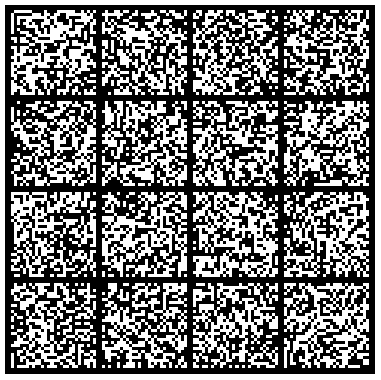
\includegraphics[scale=0.3]{img/vae_sample_0}
\end{subfigure}
\begin{subfigure}{0.32\textwidth}
\centering
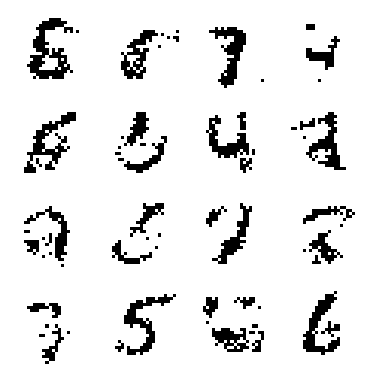
\includegraphics[scale=0.3]{img/vae_sample_20}
\end{subfigure}
\begin{subfigure}{0.32\textwidth}
\centering
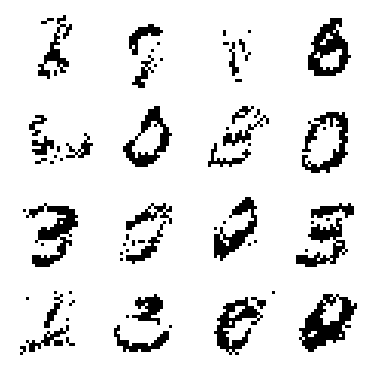
\includegraphics[scale=0.3]{img/vae_sample_40}
\end{subfigure}
 \caption{Samples from the VAE, from left to right: before training, halfway through and after training. As training progresses, the samples increasingly resemble samples from the training data.}
\label{fig:vae_samples}
\end{figure}

\subsection*{Question 1.15}

In order to visualize the latent space in the regions of significant density in a two-dimensional latent space, we map the square of probabilities $[0.05, 0.95]^2$ to values of $Z$ using the inverse CDF of the standard Gaussian distribution. This results in a grid of latent variables, which we pass through the decoder to obtain the means of the corresponding Bernoulli distributions. The results are shown in Figure \ref{fig:manifold}. We can see that the continuous latent space allows to find a smooth interpolation between the different digits in the dataset.

\begin{figure}[t]
\centering
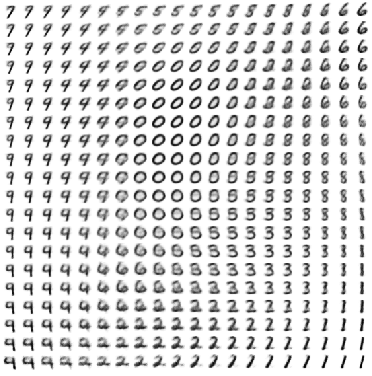
\includegraphics[scale=0.8]{img/manifold}
\caption{Data manifold learned by the VAE. Values in a grid of a 2-dimensional latent space are mapped by the decoder to the respective means of the Bernoulli distribution.}
\label{fig:manifold}
\end{figure}

\section{Generative Adversarial Networks}

\subsection*{Question 2.1}

The input of the generator is a noise sample from a prior distribution. The output is a vector in the data space. For the generator, the input is a vector in the data space, which might come from either the training data, or the generator. The output is a single number representing the probability that the input comes from the training data.

\subsection*{Question 2.2}

\begin{itemize}
\item $\mathbb{E}_{p_{\text{data}}(\mathbf{x})}[\log D(X)]$ is the expected log-probability of a \textit{real} sample that the discriminator assigns to observations from the training data. By maximizing this term with respect to $D$, we make the discriminator to correctly recognize samples from the training term.
\item $\mathbb{E}_{p_{\mathbf{z}}(\mathbf{z})}[\log (1-D(G(Z)))]$ is the expected log-probability of a \textit{fake} sample that the discriminator assigns to observations from the generator network. Minimizing this term with respect to $D$ allows the discriminator to detect images from the generator that are disparate from samples in the training data.
\end{itemize}

\subsection*{Question 2.3}

Assuming that at convergence the generator has matched the data distribution, the discriminator has no better choice than to predict a probability of $\tfrac{1}{2}$ everywhere \cite{goodfellow2014generative}. The value of $V(D, G)$ at convergence is thus $\log\tfrac{1}{2} + \log\tfrac{1}{2} = -\log 4$.

\subsection*{Question 2.4}

Early on during training, the generator has not been trained enough to produce samples similar to those in the training data. In this case it is easier for the discriminator to learn to distinguish between real and fake samples, so the term $\log (1-D(G(Z)))$ will be close to zero no matter how good $G$ is, and too small gradients, if any, will be available to update the parameters of the generator.

To solve this, the minimax game can be modified with the following equivalent objective:

\begin{equation}
\max_G \max_D \mathbb{E}_{p_{\text{data}}(\mathbf{x})}[\log D(X)] + \mathbb{E}_{p_{\mathbf{z}}(\mathbf{z})}[\log D(G(Z)]
\end{equation}

This objective is equivalent because we now find $G$ to maximize the probability that $D$ makes a mistake by identifying a fake sample as real. The advantage from the point of view of gradient-based learning is that the term $\log D(G(Z)$ will tend to $-\infty$ the more $D$ is a good discriminator and $G$ a bad generator, thus providing better gradients for updating $G$.




























\bibliographystyle{unsrt}
\bibliography{refs}
\end{document}
